\chapter{Configuration}
\label{chap-user}

\renewcommand{\headrulewidth}{0.3pt}
\fancyhead[LE]{\thepage} \fancyhead[RE]{\nouppercase{\textbf{\leftmark}}}
\fancyhead[RO]{\thepage} \fancyhead[LO]{\nouppercase{\textbf{\rightmark}}}
\fancyfoot[L,C,R]{}

\setlength{\parindent}{0.35cm}

\minitoc
\newpage
% ================================================================

\section{Overview}
\label{sec-generalites}

The \cwv~extension integrates several features accessible from its home dialog box (\cref{fig-cwv_home_page}):
\begin{itemize}
    \item a dedicated entry for configuring the \cawaqs~application (\gui{Settings}
        - \cref{sec_config} to \ref{sec-json_config_project}) ;

    \item calibration assistance tools (\gui{Calibration tools} - \cref{sec-calib-tools})
        ;

    \item features for visualizing simulated and observed flow and piezometry time series (\gui{Compare Sim/Obs} - \cref{sec-com-simobs})
        ;

    \item tools for visualizing the spatial distribution of hydrological components
        (\gui{Spatial Maps} - \cref{sec-spatial-map}) ;

    \item a hydrological budget visualization function (\gui{Budget Bar Plot}
        - \cref{sec-bufget-barplot}) ;

    \item a hydrological regime viewer (\gui{Hydrological regime} - \cref{sec-regime-hydro}).
\end{itemize}

\begin{figure}[H]
    \centering
    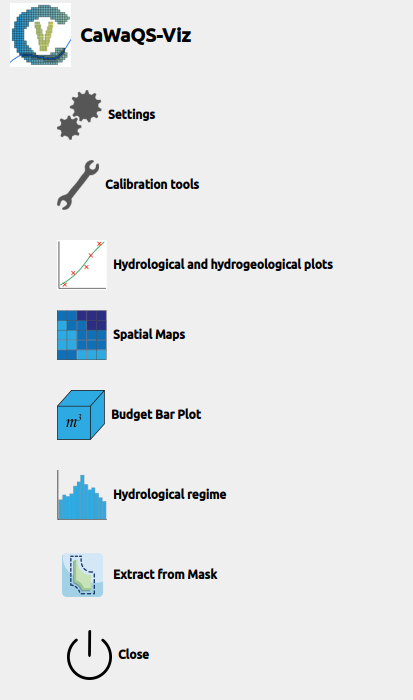
\includegraphics[width=0.4\linewidth]{
        2_application_user_guide/fig/CAWAQS_VIZ_home_page.png
    }
    \caption{Home dialog box of the \cwv~application.}
    \label{fig-cwv_home_page}
\end{figure}

The use of the \cwv~extension is based on a pre-existing \script{GIS} project
containing:
\begin{itemize}
    \item the meshes of the various \cawaqs~application modules, at the
        modelling output resolutions;

    \item observation points and/or extraction points, located within the bounds of the model extent.
\end{itemize}

\subsection{Mode of \cwv~Configuration}
\label{sec_config}

The plug-in must be configured to read the various modelling output files
and/or \cawaqs~input files as well as the various meshes. This parameterisation
of the plug-in can be carried out in the \gui{Settings} window. To do so, two
procedures are available \ref{fig-DialogSettings}:
\begin{itemize}
     \item FIRST TIME: configure the project manually in the second part of the dialog box (section \ref{sec-auto-detection}).
    \item ALREADY SET: import a \script{.json} configuration file established beforehand (section \ref{sec-json_config_project}).;

\end{itemize}

\begin{figure}[H]
    \centering
    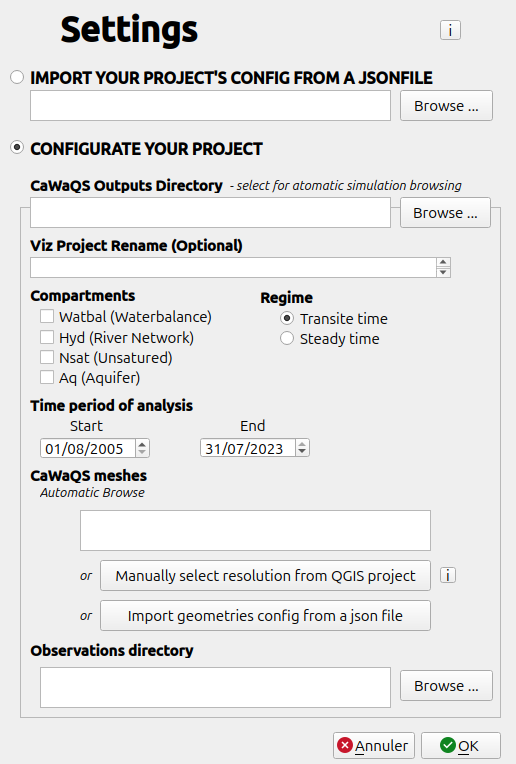
\includegraphics[width=0.45\linewidth]{
        2_application_user_guide/fig/DialogSettings.png
    }
    \caption{The \gui{Settings} dialog box of the plug-in, selecte the creation of a new project.}
    \label{fig-DialogSettings}
\end{figure}

The details of these two application configuration procedures are described
in paragraphs \ref{sec-auto-detection} and \ref{sec-json_config_project} respectively.

% ================================================================
% Automatic detection of project settings from the file system.
% Standalone section — uses the guide's shortcuts (\cwv, \cawaqs,
% \gui, \script) and the json lstlisting language defined in main_ENG.tex.
% Drop into Chap2 with \input, or \include as its own file.
% ================================================================

\section{Automatic Detection of Project Settings}
\label{sec-auto-detection}

When configuring a project manually (rather than importing a
\script{.json} configuration file), \cwv~can pre-fill most of the
\gui{Settings} dialog by inspecting the file system. The only action
required from the user is to browse to the \cawaqs~output directory:
detection then runs automatically and fills in the compartments, the
simulation years, the regime, the observation directory and the
geometry configuration path.

Detection is a \emph{best-effort} convenience. It relies entirely on the
naming and layout conventions described below. If a convention is not
met, the corresponding field is simply left empty and can be filled by
hand — the only hard requirement is that the output directory contain at
least one recognisable module sub-folder (see \cref{ssec-auto-outcaw}).

Detection is driven by two independent probes anchored on two different
roots:
\begin{itemize}
    \item the \cawaqs~\textbf{output directory} you select
        (\cref{ssec-auto-outcaw}) — drives the compartments, years and
        regime;

    \item the \textbf{QGIS project file} (\script{.qgz}~/~\script{.qgs})
        currently open (\cref{ssec-auto-neighbors}) — drives the
        geometry configuration, the observation directory and the
        project name.
\end{itemize}

% ----------------------------------------------------------------
\subsection{Probe 1 — from the \cawaqs~output directory}
\label{ssec-auto-outcaw}

This probe is anchored on the output directory selected through the
\gui{Browse} button. It expects, directly inside that directory, one or
more module output sub-folders, each named after its \cawaqs~module:

\begin{center}
\begin{tabular}{ll}
    \textbf{Sub-folder} & \textbf{Detected compartment} \\
    \hline
    \script{Output\_AQ}      & \script{AQ} (aquifers)        \\
    \script{Output\_HYD}     & \script{HYD} (hydraulic network) \\
    \script{Output\_WATBAL}  & \script{WATBAL} (surface water balance) \\
    \script{Output\_NONSAT}  & \script{NSAT} (unsaturated zone) \\
\end{tabular}
\end{center}

At least one of these sub-folders must be present; otherwise detection
fails and the dialog must be filled manually.

Inside each module sub-folder, the \textbf{binary result filenames}
determine the simulation years and the regime. Two filename patterns are
recognised:

\begin{itemize}
    \item \script{<MODULE>\_<VAR>.YYYYYYYY.bin} — a \textbf{transient}
        yearly step. The eight digits encode two consecutive years, the
        start \script{YYYY} followed by the end \script{YYYY}, where the
        end is the start $+\,1$ (e.g. \script{20102011}). Each such file
        contributes its start year; the earliest start and the latest
        end define the simulation range.

    \item \script{<MODULE>\_<VAR>.00.bin} — a \textbf{steady-state}
        result. The presence of this pattern marks the run as steady.
\end{itemize}

The regime is resolved as follows: \script{Steady} if only steady
filenames are found and no transient ones; otherwise \script{Transient}.
If both patterns coexist, the run is classified as \script{Transient}
and a warning is issued. If no year could be read from any filename, the
range defaults to \script{1970}--\script{2022}.

The expected disposition therefore looks like:

\begin{lstlisting}[caption={Expected layout of the \cawaqs~output directory.},captionpos=b,frame=lines,basicstyle=\ttfamily\footnotesize]
<OUT_CAW>/
|-- Output_AQ/
|     |-- AQ_HEAD.20102011.bin      <-- transient (2010->2011)
|     |-- AQ_HEAD.20112012.bin      <-- transient (2011->2012)
|     +-- ...
|-- Output_HYD/
|     +-- HYD_Q.20102011.bin
|-- Output_WATBAL/
|     +-- WATBAL_...00.bin          <-- steady-state token
+-- Output_NONSAT/
      +-- ...
\end{lstlisting}

\alertinfo{The regime, the compartment list and the simulation years are
    read \emph{only} from this probe. Browsing to the output directory is
    thus the single mandatory step for automatic detection.}

% ----------------------------------------------------------------
\subsection{Probe 2 — from the QGIS project neighbours}
\label{ssec-auto-neighbors}

This probe is anchored on the currently open QGIS project file
(\script{.qgz}~/~\script{.qgs}). It is purely best-effort: each of the
three items below is looked up independently, and any of them may remain
empty without preventing detection.

\begin{itemize}
    \item \textbf{Geometry configuration} — the probe searches for files
        matching \script{config\_geometries\_*.json} in the \emph{same
        folder} as the project file. If several match, the most recently
        modified one is used.

    \item \textbf{Observation directory} — the probe looks for a folder
        named \script{DATA\_OBS} at the level of the project file, then
        one level up, then two levels up, and stops at the first match.

    \item \textbf{Project name} — derived from the folder that
        \emph{contains} \script{DATA\_OBS} when it is found; otherwise
        from the project file's parent (or grand-parent) folder name.
\end{itemize}

The expected neighbourhood of the project file is:

\begin{lstlisting}[caption={Expected layout around the QGIS project file.},captionpos=b,frame=lines,basicstyle=\ttfamily\footnotesize]
<project_root>/                     <-- name used as project name
|-- DATA_OBS/                       <-- observation directory
+-- <qgis_folder>/
      |-- my_project.qgz            <-- open QGIS project
      +-- config_geometries_*.json  <-- geometry config (newest wins)
\end{lstlisting}

\alertwarning{Because the geometry configuration is searched only next
    to the \script{.qgz}~/~\script{.qgs} file, and \script{DATA\_OBS} only
    up to two levels above it, a project saved outside its usual folder
    structure will leave these fields empty. This is expected — fill them
    manually via the \gui{Configure Geometry} button and the observation
    browse field.}

% ----------------------------------------------------------------



\section{Project Configuration from a \json~File}
\label{sec-json_config_project}

Once a project has been configured (whether by automatic detection or by
hand), its configuration is written as \script{.json} files under
\script{<OUT\_CAW>/PostProcessing/CONFIG/}, namely
\script{config\_project\_<name>.json} and
\script{config\_geometries\_<name>.json}. These files can later be
re-imported directly through the first configuration procedure, bypassing
detection entirely. 

Importing an external \json~file can also be used to configure
the project. This file is automatically saved into the Postprocessing directory of a project after its first configuration. 

Upon execution of the \cwv~application parameterisation dialog box, the
project sub-directory is created in the specified post-processing directory.
If the project does not yet exist in this directory, a sub-directory named after
the project will be created, containing the project and resolution configuration files
written in \gui{json} format.


 This project configuration \json~file is structured as follows:

\begin{lstlisting}[language=json]
{
    "json_path_geometries": str,
    "projectName": str, 
    "cawOutDirectory": str,
    "startSim": int,
    "endSim": int,
    "obsDirectory": str,
    "ppDirectory": str, 
    "regime": str
}
\end{lstlisting}

\vspace{-0.6cm}
The contents of each object in this \json~file are as follows:
\begin{itemize}
    \item \gui{json\_path\_geometries}: absolute path of the resolution
        configuration file;

    \item \gui{projectName}: project name;

    \item \gui{cawOutDirectory}: absolute path of the directory containing the
        \cawaqs~modelling outputs;

    \item \gui{startSim} and \gui{endSim}: simulation start and end years
        in \script{integer} format;

    \item \gui{obsDirectory}: absolute path of the parent directory containing the
        observed time series;

    \item \gui{ppDirectory}: absolute path of the post-processing directory. Note
        that the path must already exist. Otherwise, it will not be
        created by the application.

    \item \gui{regime}: modelling regime ("Transient" or "Steady")
\end{itemize}
